\documentclass{beamer}
\usetheme{tokitex}

\usepackage{graphics}
\usepackage{multirow}
\usepackage{tabto}

\usepackage[english,bahasa]{babel}
\newtranslation[to=bahasa]{Section}{Bagian}
\newtranslation[to=bahasa]{Subsection}{Subbagian}

\usepackage{listings, lstautogobble}
\usepackage{color}

\definecolor{dkgreen}{rgb}{0,0.6,0}
\definecolor{gray}{rgb}{0.5,0.5,0.5}
\definecolor{mauve}{rgb}{0.58,0,0.82}

\lstset{frame=tb,
  language=pascal,
  aboveskip=1mm,
  belowskip=1mm,
  showstringspaces=false,
  columns=fullflexible,
  keepspaces=true,
  basicstyle={\small\ttfamily},
  numbers=none,
  numberstyle=\tiny\color{gray},
  keywordstyle=\color{blue},
  commentstyle=\color{dkgreen},
  stringstyle=\color{mauve},
  breaklines=true,
  breakatwhitespace=true,
  autogobble=true
}

\title{Pengurutan}
\author{Tim Olimpiade Komputer Indonesia}
\date{}

\begin{document}

\begin{frame}
\titlepage
\end{frame}

\begin{frame}
\frametitle{Pendahuluan}
Melalui dokumen ini, kalian akan:
\begin{itemize}
  \item Mempelajari konsep algoritma sederhana.
  \item Memahami berbagai algoritma pengurutan sederhana.
  \item Memahami keuntungan dan kerugian dari masing-masing algoritma.
\end{itemize}
\end{frame}

\begin{frame}
\frametitle{Pendahuluan (lanj.)}
\begin{itemize}
  \item Pengurutan sering digunakan dalam pemrograman untuk membantu membuat data lebih mudah diolah.
  \item Terdapat berbagai macam cara untuk melakukan pengurutan,
  masing-masing dengan keuntungan dan kekurangannya.
\end{itemize}
\end{frame}

\begin{frame}
\frametitle{Soal: Bebek Berbaris}
Deskripsi:
\begin{itemize}
  \item Sebelum masuk ke dalam kandang, para bebek akan berbaris terlebih dahulu.
  \item Seiring dengan berjalannya waktu, bebek-bebek tumbuh tinggi. Pertumbuhan ini berbeda-beda; ada bebek yang lebih tinggi dari bebek lainnya.
  \item Terdapat $N$ ekor bebek, bebek ke-$i$ memiliki tinggi sebesar $h_i$.
  \item Perbedaan tinggi ini menyebabkan barisan terlihat kurang rapi, sehingga Pak Dengklek ingin bebek-bebek berbaris dari yang paling pendek ke paling tinggi.
  \item Bantulah para bebek untuk mengurutkan barisan mereka!
\end{itemize}
\end{frame}

\begin{frame}
\frametitle{Soal: Bebek Berbaris (lanj.)}
%Format masukan:
%\begin{itemize}
%  \item Baris pertama berisi sebuah bilangan bulat, yaitu $N$.
%  \item Baris kedua berisi $N$ bilangan bulat. Bilangan ke-$i$ menyatakan $h_i$.
%\end{itemize}
%Format keluaran:
%\begin{itemize}
%  \item Keluarkan ketinggian bebek dalam keadaan terurut menaik, seekor bebek pada setiap barisnya.
%\end{itemize}
  Batasan:
  \begin{itemize}
    \item $1 \le N \le 1.000$
    \item $1 \le h_i \le 100.000$, untuk $1 \le i \le N$
  \end{itemize}
\end{frame}


\begin{frame}
\frametitle{Solusi}
  \begin{itemize}
    \item Persoalan ini meminta kita melakukan pengurutan $N$ bilangan dengan rentang datanya antara $1$ sampai $100.000$.
    \item Terdapat sejumlah algoritma pengurutan, yang akan dibahas pada bagian berikutnya.
  \end{itemize}
\end{frame}

\section{Bubble Sort}
\frame{\sectionpage}

\begin{frame}
\frametitle{Ide Dasar}
  \begin{itemize}
    \item Mulai dari elemen pertama, cek apakah elemen sesudahnya (yaitu elemen kedua) lebih kecil.
    \item Bila ya, artinya elemen pertama ini harus terletak sesudah elemen kedua. Untuk itu, lakukan penukaran.
    \item Bila tidak, tidak perlu lakukan penukaran.
    \item Lanjut periksa elemen kedua, ketiga, dan seterusnya.
  \end{itemize}
\end{frame}

\begin{frame}
\frametitle{Ide Dasar (lanj.)}
  \begin{itemize}
    \item Proses ini mengakibatkan elemen dengan nilai terbesar pasti
    digiring ke posisi terakhir:
    
    \begin{figure}
      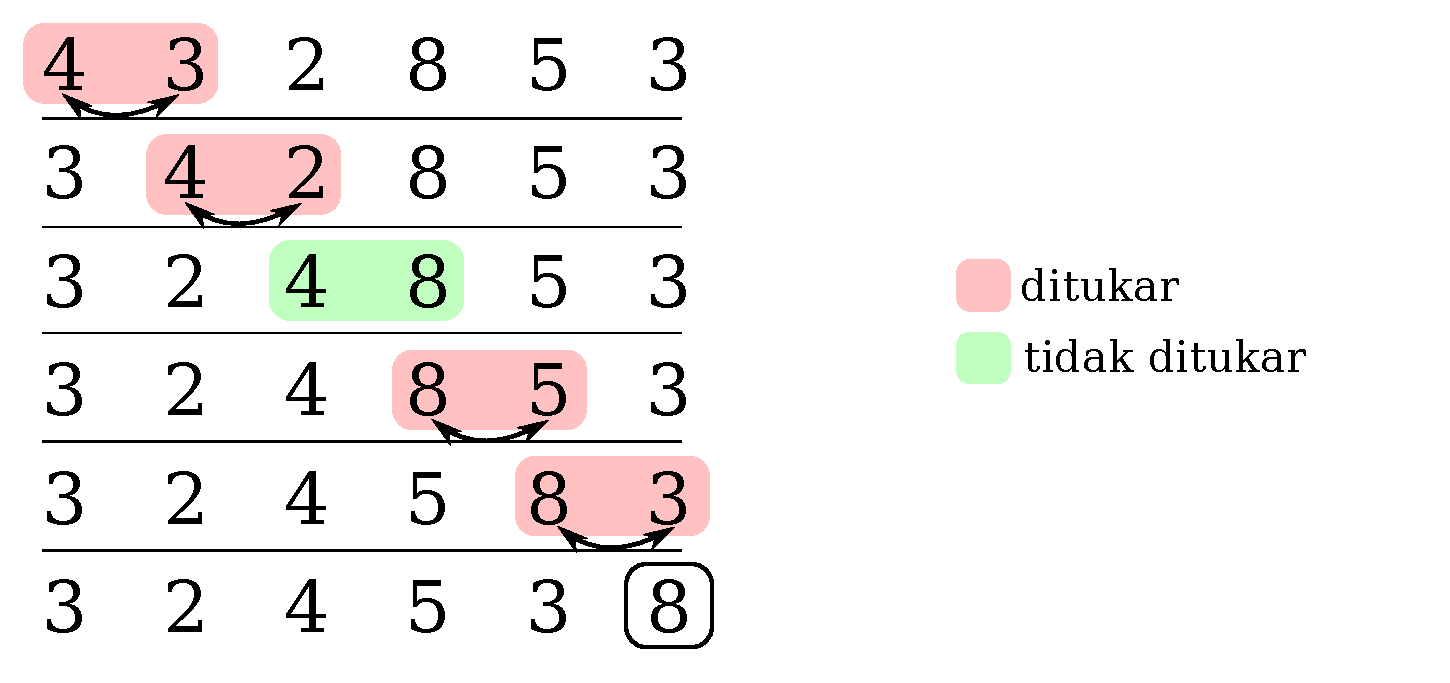
\includegraphics[width=11cm]{asset/bubble-sort-1.pdf}
    \end{figure}
  \end{itemize}
\end{frame}

\begin{frame}
\frametitle{Ide Dasar (lanj.)}
  \begin{itemize}
    \item Bila proses ini dilakukan lagi, maka elemen kedua terbesar
    akan terletak di posisi kedua dari terakhir.
    \item Kali ini pemeriksaan cukup dilakukan sampai 1 elemen
    sebelum posisi terakhir, sebab elemen terakhir sudah pasti
    tidak akan berubah posisi:
    
    \begin{figure}
      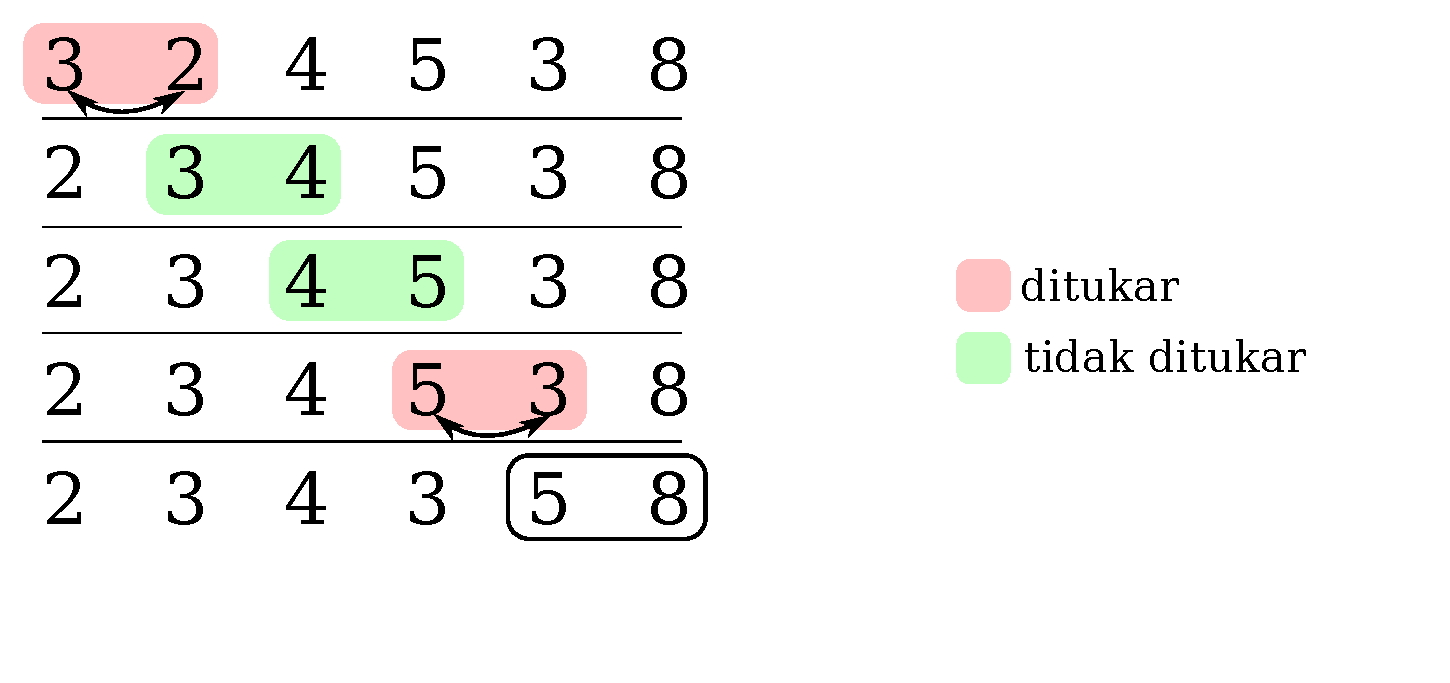
\includegraphics[width=11cm]{asset/bubble-sort-2.pdf}
    \end{figure}
  \end{itemize}
  
\end{frame}

\begin{frame}
\frametitle{Ide Dasar (lanj.)}
  \begin{itemize}
    \item Demikian pula untuk eksekusi yang ketiga kalinya, yang
    kebetulan data sudah menjadi terurut:
    \begin{figure}
      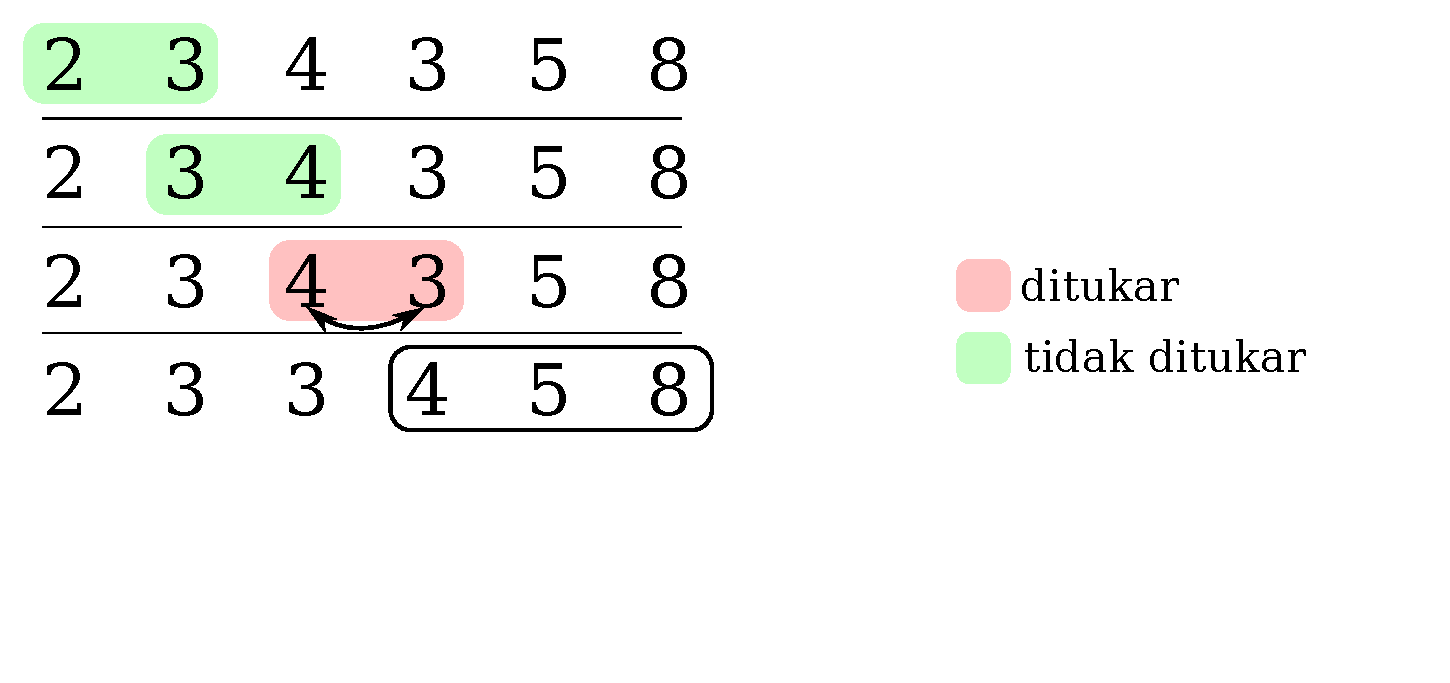
\includegraphics[width=11cm]{asset/bubble-sort-3.pdf}
    \end{figure}
  \end{itemize}
\end{frame}

\begin{frame}
\frametitle{Ide Dasar (lanj.)}
  \begin{block}{Pertanyaan}
    Jika eksekusi ke-$i$ mengakibatkan $i$ elemen terbesar terletak di $i$
    posisi terakhir, maka berapa kali eksekusi yang dibutuhkan sampai
    seluruh data dijamin terurut?
  \end{block}
\end{frame}

\begin{frame}
\frametitle{Analisis}
  \begin{itemize}
    \item Dibutuhkan $N$ kali eksekusi hingga seluruh data terurut.
    \item Dalam sekali eksekusi, dilakukan iterasi dari elemen pertama
    sampai elemen terakhir, yang kompleksitasnya berkisar antara
    $O(1)$ sampai $O(N)$, tergantung eksekusi ke berapa.
    \item Secara rata-rata, kompleksitasnya setiap eksekusi adalah
    $O(N/2)$, yang bisa ditulis $O(N)$.
    \item Total kompleksitas bubble sort adalah $O(N^2)$.
  \end{itemize}
\end{frame}

\begin{frame}[fragile]
\frametitle{Contoh Kode}
  \begin{lstlisting}
    for i := 1 to N-1 do begin
      for j := 1 to N-i do begin
        if (h[j] > h[j+1]) then begin
          swap(h[j], h[j+1]); (* tukar h[j] dengan h[j+1] *)
        end;
      end;
    end;
  \end{lstlisting}
  Catatan: fungsi \textbf{swap} tidak tersedia secara \textit{default} pada Pascal, jadi harus Anda implementasikan sendiri.
\end{frame}

\section{Selection Sort}
\frame{\sectionpage}

\begin{frame}
\frametitle{Ide Dasar}
  \begin{itemize}
    \item Pilih elemen terkecil dari data, lalu pindahkan ke elemen pertama.
    \item Pilih elemen terkecil dari data yang tersisa, lalu pindahkan ke  elemen kedua.
    \item Pilih elemen terkecil dari data yang tersisa, lalu pindahkan ke elemen ketiga.
    \item ... dan seterusnya sampai seluruh elemen terurut.
  \end{itemize}
\end{frame}

\begin{frame}
\frametitle{Ilustrasi Jalannya Algoritma}
  \begin{figure}
    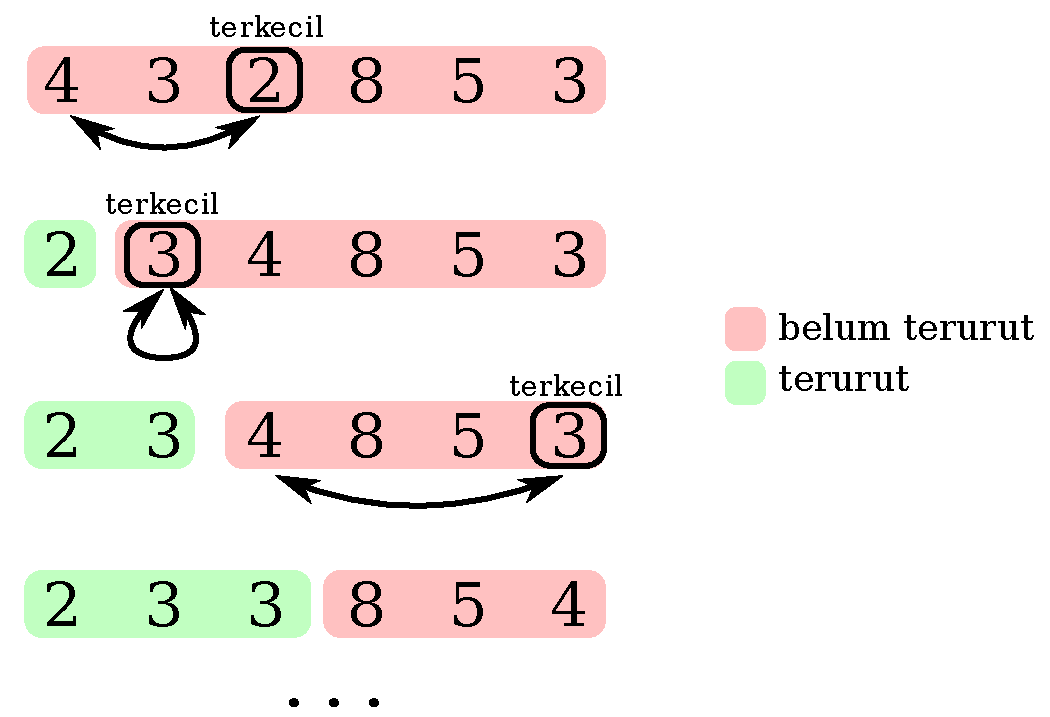
\includegraphics[width=10cm]{asset/selection-sort.pdf}
  \end{figure}
\end{frame}
    
\begin{frame}
\frametitle{Analisis}
  \begin{itemize}
    \item Pencarian elemen terkecil dapat dilakukan dengan \textit{linear search}.
    \item Berhubung perlu dilakukan $N$ kali \textit{linear search}, maka kompleksitas selection sort adalah $O(N^2)$.
  \end{itemize}
\end{frame}

\begin{frame}[fragile]
\frametitle{Contoh Kode}
  \begin{lstlisting}
    for i := 1 to N do begin
      (* pencarian indeks terkecil *)
      minIndex := i;
      for j := i+1 to N do begin
        if (h[j] < h[minIndex]) then begin
          minIndex := j;
        end;
      end;
    
      (* tukar *)
      swap(h[i], h[minIndex]);
    end;
  \end{lstlisting}
\end{frame}

\begin{frame}
\frametitle{Kegunaan Khusus}
  \begin{itemize}
    \item Cara kerja selection sort memungkinkan kita untuk melakukan
    \textit{partial sort}.
    \item Jika kita hanya tertarik dengan $K$ elemen terkecil, kita bisa
    melakukan proses seleksi dan menukar pada selection sort $K$
    kali.
    \item Dengan demikian, pencarian $K$ elemen terkecil dapat
    dilakukan dalam $O(KN)$, cukup baik apabila $K$ jauh lebih
    kecil dari $N$.
  \end{itemize}
\end{frame}

\section{Insertion Sort}
\frame{\sectionpage}

\begin{frame}
\frametitle{Ide Dasar}
  \begin{itemize}
    \item Anggap kita memiliki sebagian data yang terurut.
    \item Secara bertahap, sisipkan elemen baru ke dalam data yang sudah terurut.
    \item Penyisipan ini harus dilakukan sedemikian sehingga hasilnya tetap terurut.
    \item Misalnya saat ini data yang sudah terurut adalah [1, 2, 3, 8], lalu elemen yang akan disisipkan adalah 5, maka \\
    dihasilkan [1, 2, 3, 5, 8].
  \end{itemize}
\end{frame}

\begin{frame}
\frametitle{Jalannya Algoritma}
  Prosesnya dapat digambarkan sebagai berikut:
  \begin{table}[ht]
    \begin{tabular}{|l|l|}
      \hline Data Asal  & Data Terurut \\
      \hline [4, 3, 2, 8, 5, 3] & [] \\
      \hline [3, 2, 8, 5, 3] & [4] \\
      \hline [2, 8, 5, 3] & [3, 4] \\
      \hline [8, 5, 3] & [2, 3, 4] \\
      \hline [5, 3] & [2, 3, 4, 8] \\
      \hline [3] & [2, 3, 4, 5, 8] \\
      \hline [] & [2, 3, 3, 4, 5, 8] \\
      \hline
    \end{tabular}
  \end{table}
\end{frame}

\begin{frame}
\frametitle{Proses Penyisipan (\textit{insertion})}
  \begin{itemize}
    \item Strategi yang dapat digunakan adalah meletakkan angka yang hendak disisipkan pada bagian paling belakang, lalu digiring mundur sampai posisinya tepat.
    \item Misalnya pada kasus menyisipkan angka 3 pada data 
    
    [1, 2, 5, 8, 9]:
    
    \begin{figure}
      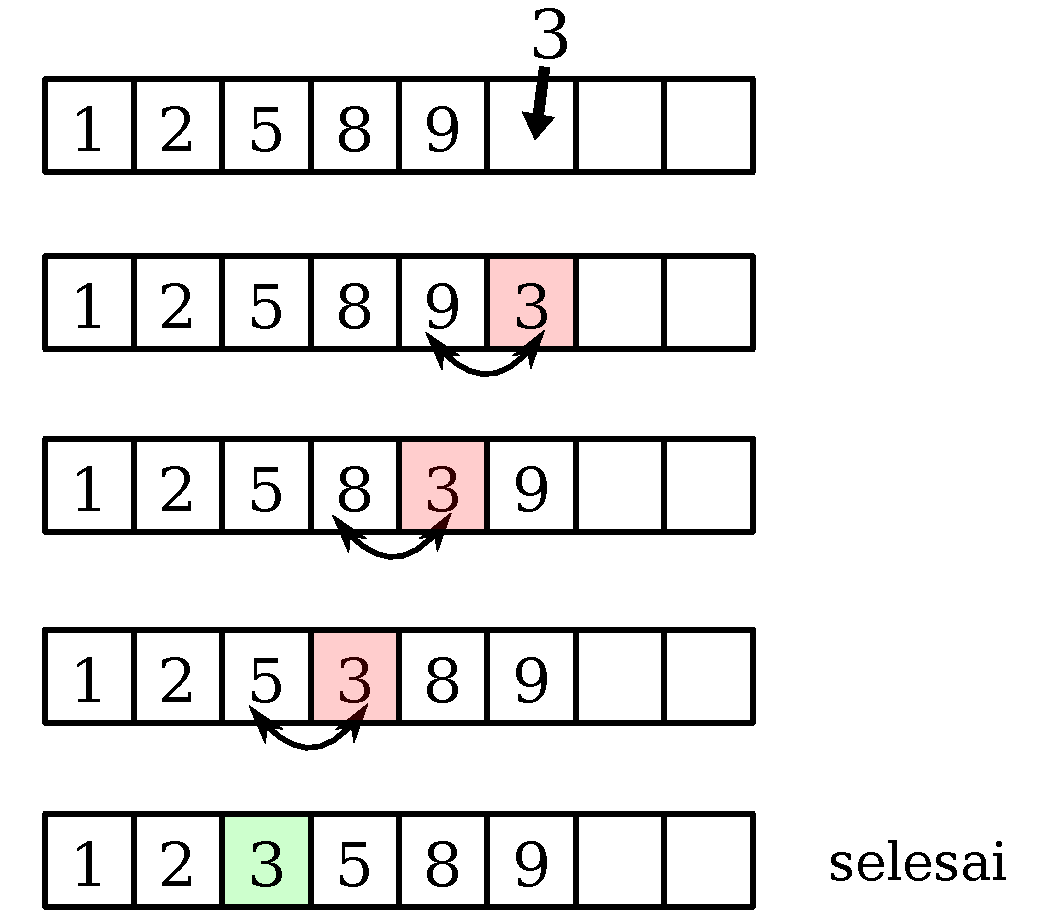
\includegraphics[width=6cm]{asset/insertion-sort-2.pdf}
    \end{figure}
  \end{itemize}
\end{frame}

\begin{frame}
\frametitle{Analisis}
  \begin{itemize}
    \item Untuk mengurutkan data, diperlukan $N$ kali penyisipan.
    \item Setiap menyisipkan, dilakukan penggiringan yang kompleksitasnya:
    \begin{itemize}
      \item Pada kasus terbaik $O(1)$, ketika angka yang dimasukkan merupakan angka terbesar pada data saat ini.
      \item Pada kasus terburuk $O(N)$, yaitu ketika angka yang dimasukkan merupakan angka terkecil pada data saat ini.
      \item Pada kasus rata-rata, kompleksitasnya $O(N/2)$, atau bisa ditulis $O(N)$.
    \end{itemize}
  \end{itemize}
\end{frame}

\begin{frame}
\frametitle{Analisis (lanj.)}
  \begin{itemize}
    \item Berdasarkan observasi tersebut, insertion sort dapat bekerja
    sangat cepat ketika datanya sudah hampir terurut.
    \item Pada kasus terbaik, insertion sort bekerja dalam $O(N)$, yaitu
    ketika data sudah terurut.
    \item Pada kasus terburuk, kompleksitasnya $O(N^2)$.
    \item Secara rata-rata, kompleksitasnya adalah $O(N^2)$.
  \end{itemize}
\end{frame}

\begin{frame}[fragile]
\frametitle{Contoh Kode}
  \begin{lstlisting}
    for i := 1 to N do begin
      pos := i;
      
      (* selama belum tepat, giring ke belakang *)
      while ((pos > 1) and (h[pos] < h[pos-1])) do begin
        swap(h[pos], h[pos-1]);
        pos := pos - 1;
      end;
    end;
  \end{lstlisting}
\end{frame}

\begin{frame}
\frametitle{Kegunaan Lain}
  \begin{itemize}
    \item Strategi \textit{insertion} pada algoritma ini dapat digunakan untuk menambahkan sebuah elemen pada data yang sudah terurut.
    \item Ketimbang mengurutkan kembali seluruh elemen, cukup
    lakukan strategi \textit{insertion} yang secara rata-rata bekerja dalam
    $O(N)$.
  \end{itemize}
\end{frame}

\section{Counting Sort}
\frame{\sectionpage}

\begin{frame}
\frametitle{Ide Dasar}
  \begin{itemize}
    \item Misalkan kita memiliki $M$ ember.
    \item Setiap ember dinomori dengan sebuah angka, yaitu mulai dari 1 sampai dengan $M$.
    \item Sebagai contoh, anggap $M$ = 5.
  \end{itemize}  
  \begin{figure}
    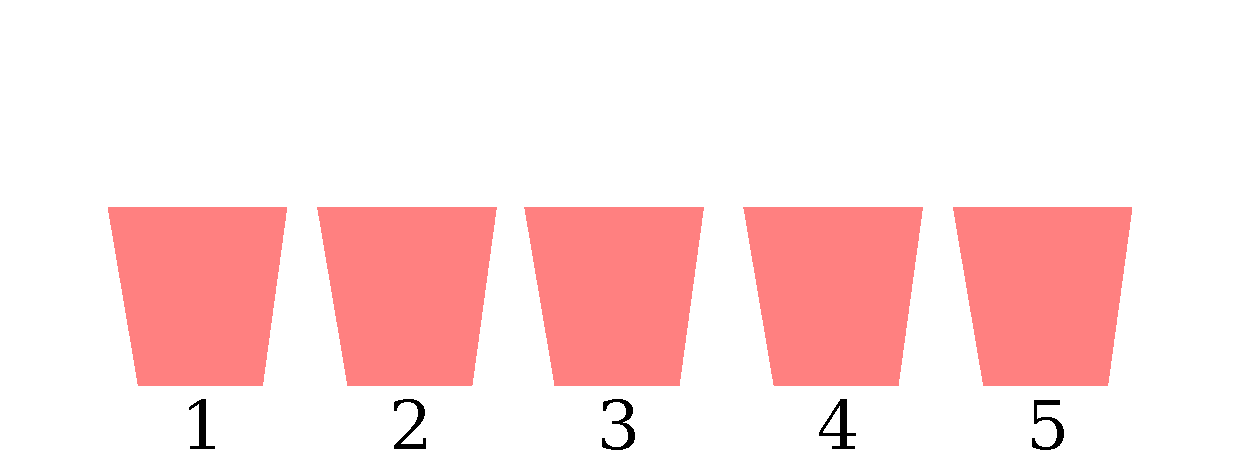
\includegraphics[width=10cm]{asset/counting-sort-1.pdf}
  \end{figure}
\end{frame}

\begin{frame}
\frametitle{Ide Dasar (lanj.)}
  \begin{itemize}
    \item Untuk setiap elemen yang mau diurutkan, masukkan ke ember yang
    sesuai dengan nilai elemen tersebut.
  \end{itemize}
  \begin{figure}
    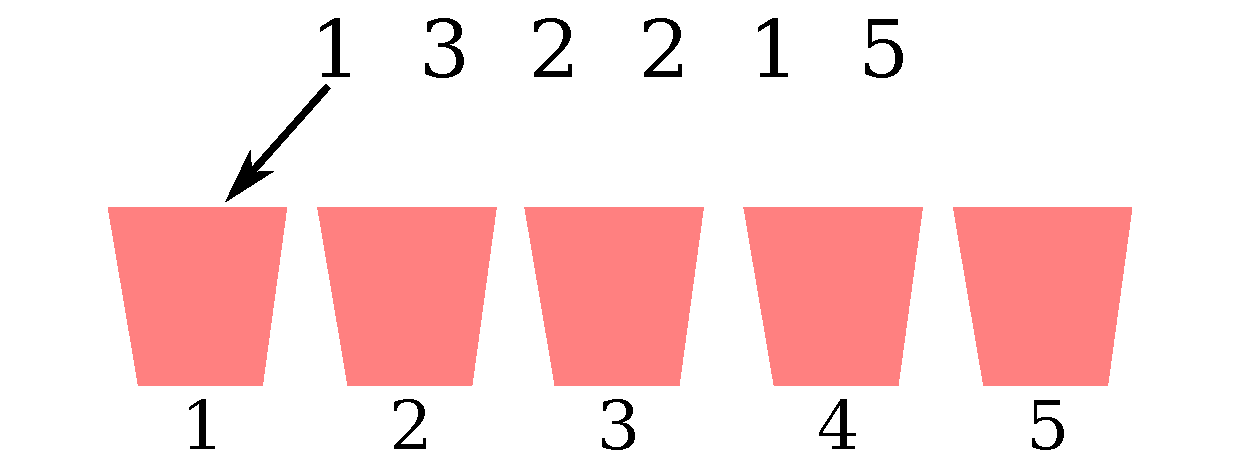
\includegraphics[width=10cm]{asset/counting-sort-2.pdf}
  \end{figure}
\end{frame}

\begin{frame}
\frametitle{Ide Dasar (lanj.)}
  \begin{itemize}
    \item Untuk setiap elemen yang mau diurutkan, masukkan ke ember yang
    sesuai dengan nilai elemen tersebut.
  \end{itemize}
  \begin{figure}
    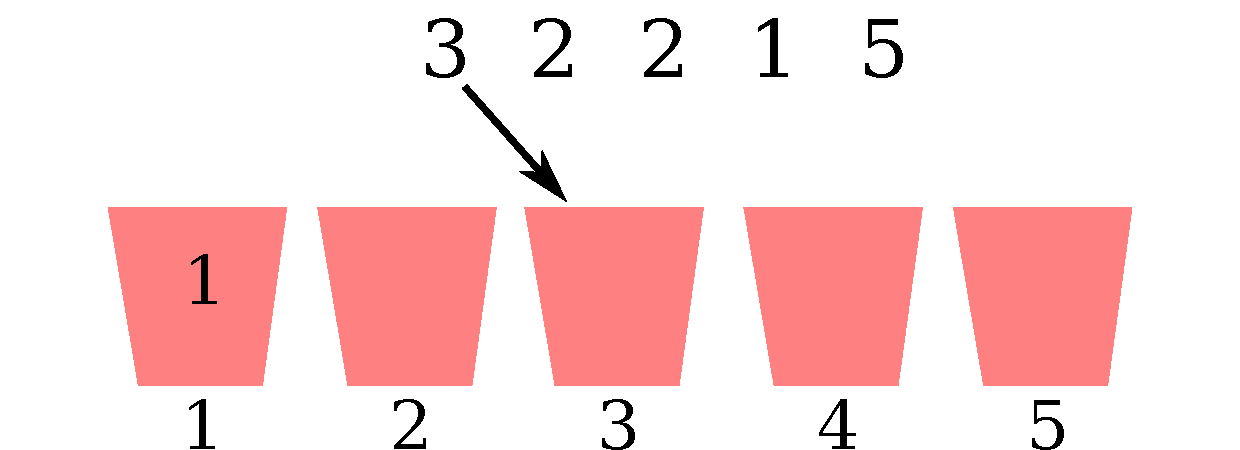
\includegraphics[width=10cm]{asset/counting-sort-3.pdf}
  \end{figure}
\end{frame}

\begin{frame}
\frametitle{Ide Dasar (lanj.)}
  \begin{itemize}
    \item Untuk setiap elemen yang mau diurutkan, masukkan ke ember yang
    sesuai dengan nilai elemen tersebut.
  \end{itemize}
  \begin{figure}
    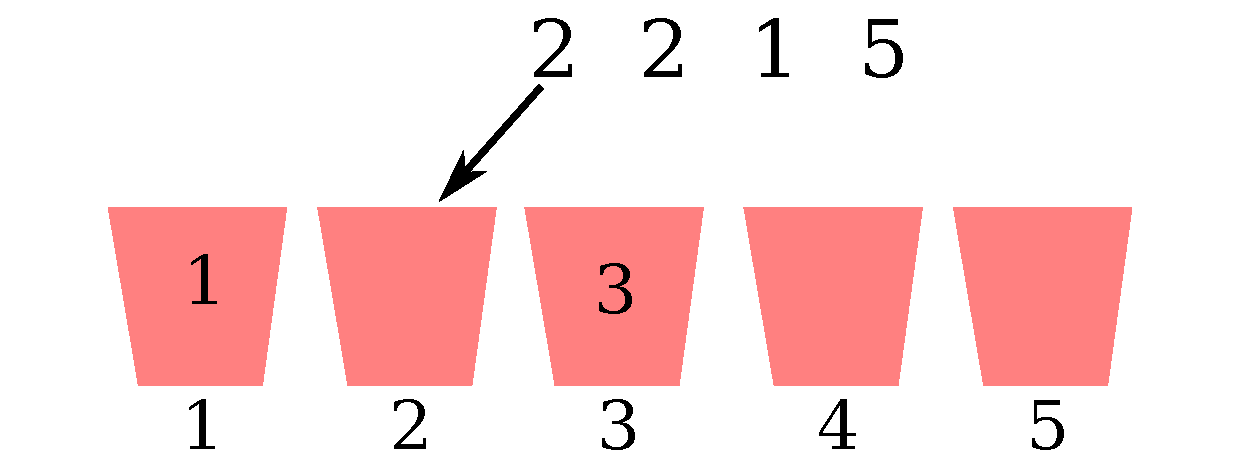
\includegraphics[width=10cm]{asset/counting-sort-4.pdf}
  \end{figure}
\end{frame}

\begin{frame}
\frametitle{Ide Dasar (lanj.)}
  \begin{itemize}
    \item Untuk setiap elemen yang mau diurutkan, masukkan ke ember yang
    sesuai dengan nilai elemen tersebut.
  \end{itemize}
  \begin{figure}
    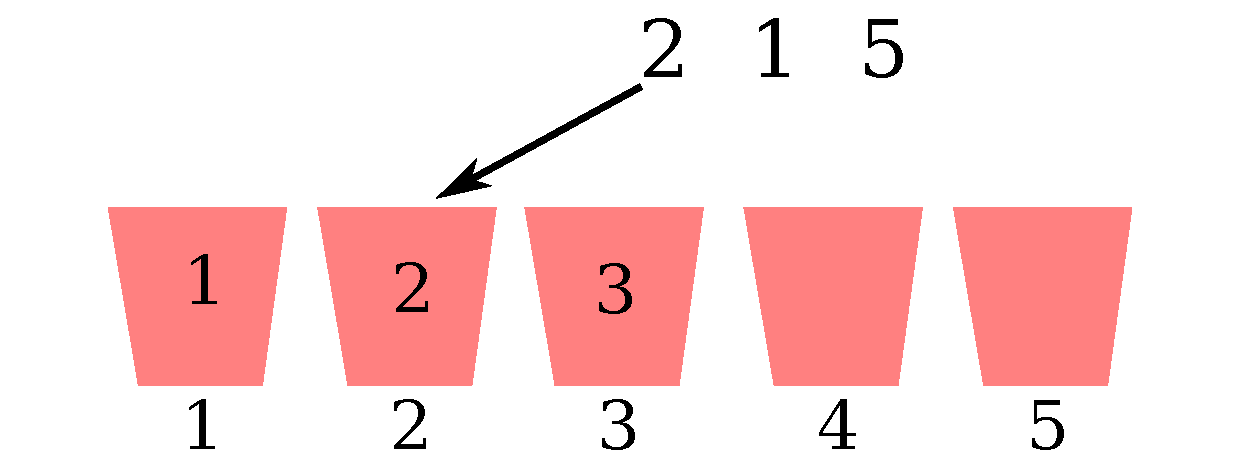
\includegraphics[width=10cm]{asset/counting-sort-5.pdf}
  \end{figure}
\end{frame}

\begin{frame}
\frametitle{Ide Dasar (lanj.)}
  \begin{itemize}
    \item Untuk setiap elemen yang mau diurutkan, masukkan ke ember yang
    sesuai dengan nilai elemen tersebut.
  \end{itemize}
  \begin{figure}
    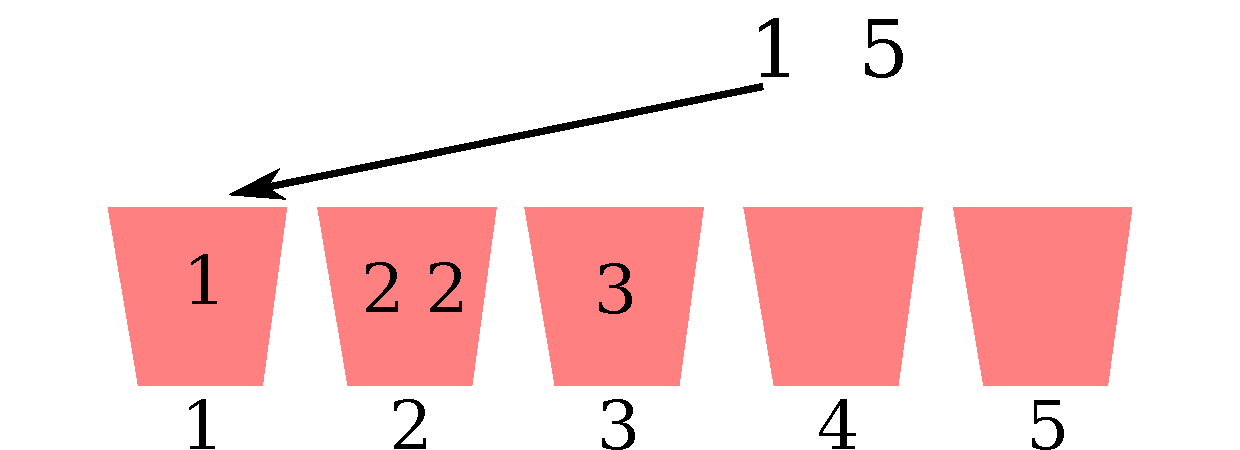
\includegraphics[width=10cm]{asset/counting-sort-6.pdf}
  \end{figure}
\end{frame}

\begin{frame}
\frametitle{Ide Dasar (lanj.)}
  \begin{itemize}
    \item Untuk setiap elemen yang mau diurutkan, masukkan ke ember yang
    sesuai dengan nilai elemen tersebut.
  \end{itemize}
  \begin{figure}
    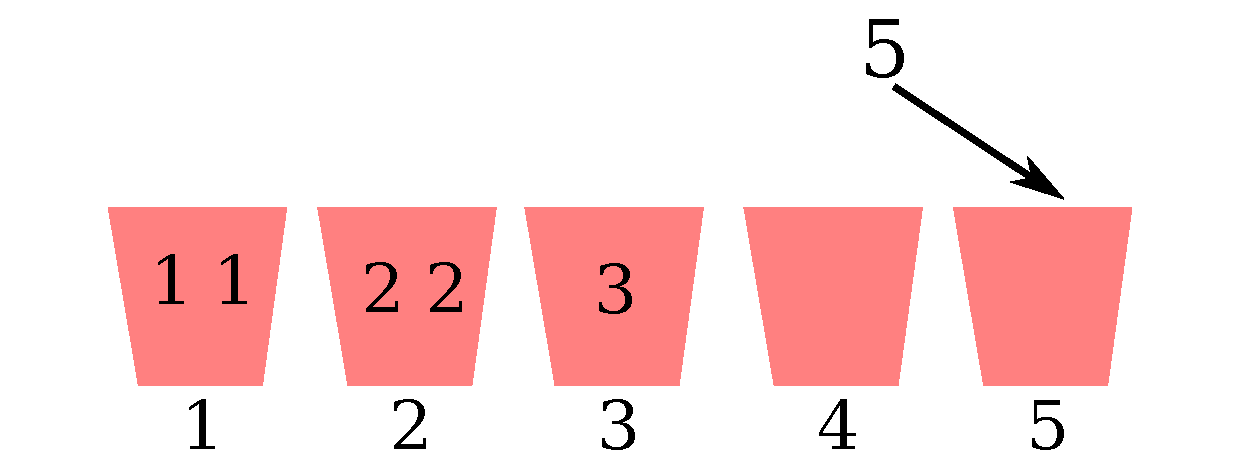
\includegraphics[width=10cm]{asset/counting-sort-7.pdf}
  \end{figure}
\end{frame}

\begin{frame}
\frametitle{Ide Dasar (lanj.)}
  \begin{itemize}
    \item Untuk setiap elemen yang mau diurutkan, masukkan ke ember yang
    sesuai dengan nilai elemen tersebut.
  \end{itemize}
  \begin{figure}
    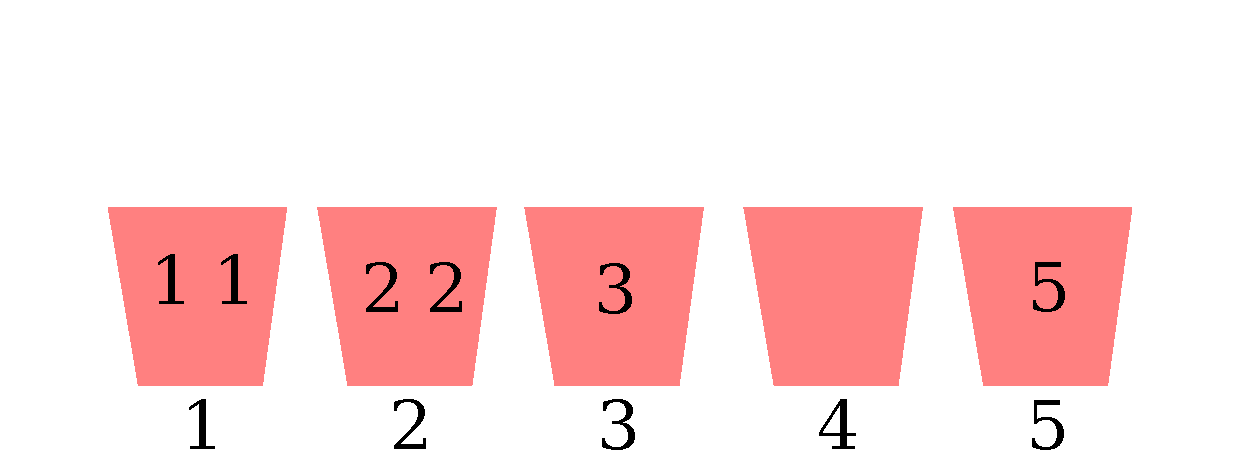
\includegraphics[width=10cm]{asset/counting-sort-8.pdf}
  \end{figure}
\end{frame}

\begin{frame}
\frametitle{Ide Dasar (lanj.)}
  \begin{itemize}
    \item Setelah seluruh elemen dimasukkan ke ember yang
    bersesuaian, keluarkan isi ember-ember mulai dari ember 1
    sampai $M$ secara berurutan.
  \end{itemize}
  \begin{figure}
    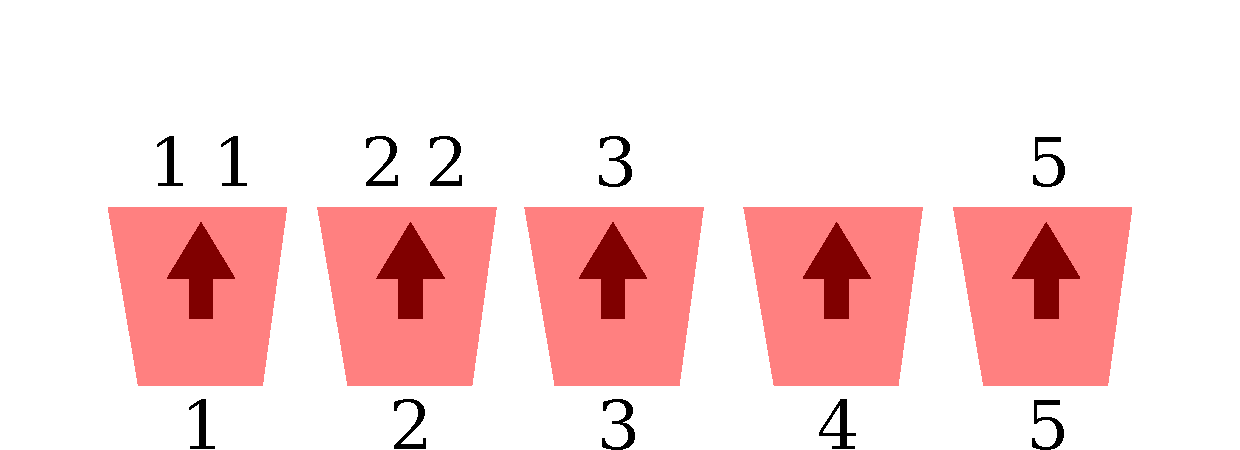
\includegraphics[width=10cm]{asset/counting-sort-9.pdf}
  \end{figure}
\end{frame}

\begin{frame}
\frametitle{Ide Dasar (lanj.)}
  \begin{itemize}
    \item Kini didapatkan data yang telah terurut.
  \end{itemize}
  \begin{figure}
    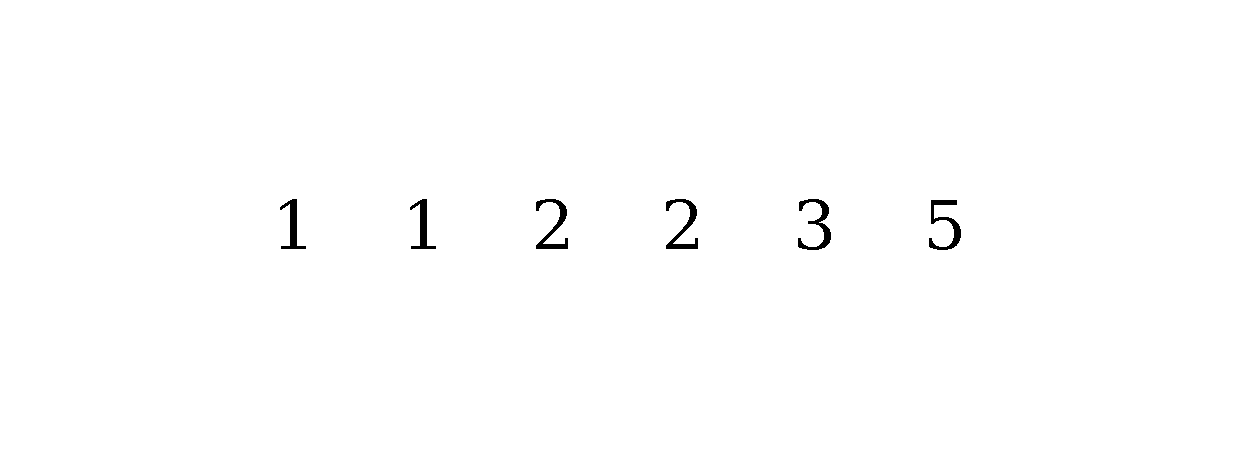
\includegraphics[width=10cm]{asset/counting-sort-10.pdf}
  \end{figure}
\end{frame}

\begin{frame}
\frametitle{Implementasi}
  \begin{itemize}
    \item Ide ini dapat diwujudkan dengan menyiapkan tabel frekuensi yang berperan sebagai ”ember”.
    \item Untuk setiap nilai elemen yang mungkin, catat frekuensi kemunculannya.
    \item Terakhir, iterasi tabel frekuensi dari elemen terkecil sampai elemen terbesar.
  \end{itemize}
\end{frame}

\begin{frame}[fragile]
\frametitle{Contoh Kode}
  \begin{itemize}
    \item Tabel frekuensi dapat diimplementasikan dengan array
    sederhana.
  \end{itemize}
  \begin{lstlisting}
    var
      ftable: array[1..100000] of longint;
      ...
    
    begin
      ...
    
      (* catat frekuensinya *)
      for i := 1 to N do begin
        x := h[i];
        ftable[x] := ftable[x] + 1;
      end;
  \end{lstlisting}
\end{frame}

\begin{frame}[fragile]
\frametitle{Contoh Kode (lanj.)}
  \begin{lstlisting}[gobble=4]
      (* tuang kembali ke h[] *)
      index := 1;
      for i := 1 to 100000 do begin
        for j := 1 to ftable[i] do begin
          h[index] := i; (* timpa h[] dengan data terurut *)
          index := index + 1;
        end;
      end;
    
      ...
    end.
  \end{lstlisting}
\end{frame}

\begin{frame}
\frametitle{Analisis}
  \begin{itemize}
    \item Dapat diperhatikan bahwa kompleksitas counting sort adalah $O(N + M)$, dengan $M$ adalah rentang nilai data.
    \item Jika $M$ tidak terlalu besar, maka counting sort dapat bekerja dengan sangat cepat.
    \item Lebih tepatnya, counting sort merupakan opsi yang sangat baik jika datanya memiliki rentang yang kecil, misalnya data tentang usia penduduk yang rentangnya hanya [0, 125].
    \item Bandingkan dengan algoritma pengurutan lain yang kompleksitasnya $O(N^2)$!
  \end{itemize}
\end{frame}

\begin{frame}
\frametitle{Kekurangan}
  \begin{itemize}
    \item Karena perlu membuat tabel frekuensi, maka counting sort hanya dapat digunakan ketika rentang nilai datanya kecil, misalnya $\le 10^7$.
    \item Selain itu, algoritma ini hanya dapat mengurutkan data diskret. Data seperti bilangan pecahan tidak dapat diurutkan secara tepat.
  \end{itemize}
\end{frame}

\begin{frame}
\frametitle{Pengembangan Counting Sort}
  \begin{itemize}
    \item Dengan adanya keterbatasan ini, counting sort dikembangkan
    menjadi radix sort.
    \item Pembelajaran tentang radix sort akan dilakukan pada
    kesempatan yang lain.
    \item Bila Anda tertarik, Anda dapat mempelajarinya \href{https://en.wikipedia.org/wiki/Radix_sort}{\textbf{di sini}}.
  \end{itemize}
\end{frame}

\begin{frame}
\frametitle{Rangkuman}
  \begin{table}[ht]
    \begin{tabular}{|l|l|p{5 cm}|}
      \hline Algoritma  & Kompleksitas & Keterangan \\
      \hline Bubble Sort & $O(N^2)$ & - \\
      \hline Selection Sort & $O(N^2)$ & Dapat digunakan untuk \textit{partial sort} dalam $O(KN)$ \\
      \hline Insertion Sort & $O(N^2)$ & Sangat cepat jika data hampir terurut, kasus terbaiknya $O(N)$ \\
      \hline Counting Sort & $O(N+M)$ & Cepat hanya untuk data dengan rentang yang kecil \\
      \hline
    \end{tabular}
  \end{table}
\end{frame}

\begin{frame}
\frametitle{Catatan}
  \begin{itemize}
    \item Terdapat algoritma pengurutan yang lebih efisien, misalnya Quicksort dan Merge Sort.
    \item Algoritma pengurutan lanjut akan dipelajari pada kesempatan yang lain.
  \end{itemize}
\end{frame}

\end{document}
